\documentclass[convert={density=300,size=400x300,outext=.png}]{standalone}
\usepackage{tikz}

\thispagestyle{empty}

\begin{document}
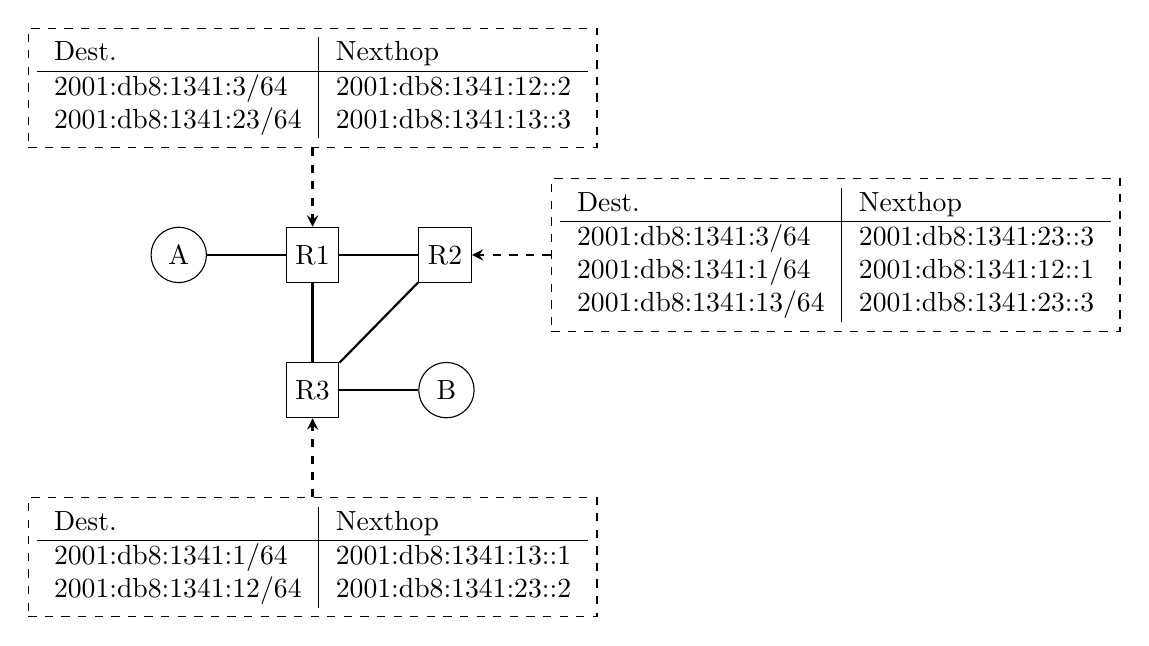
\begin{tikzpicture}
  \usetikzlibrary{positioning,matrix,arrows}
    \tikzstyle{arrow} = [thick,->,>=stealth]
       \tikzset{router/.style = {rectangle, draw, text centered, minimum height=2em}, }
       \tikzset{host/.style = {circle, draw, text centered, minimum height=2em}, }
       \tikzset{ftable/.style={rectangle, dashed, draw} }
       \node[host] (A) {A};
       \node[router, right=of A] (R1) { R1 };
       \node[ftable, above=of R1] (FR1) { \begin{tabular}{l|l} 
       Dest. & Nexthop \\
       \hline
       2001:db8:1341:3/64 & 2001:db8:1341:12::2 \\
       2001:db8:1341:23/64 & 2001:db8:1341:13::3 \\
       \end{tabular}};
       \node[router,right=of R1] (R2) {R2};
       \node[ftable, right=of R2] (FR2) { \begin{tabular}{l|l} 
       Dest. & Nexthop \\
       \hline 
       2001:db8:1341:3/64 & 2001:db8:1341:23::3 \\
       2001:db8:1341:1/64 & 2001:db8:1341:12::1 \\
       2001:db8:1341:13/64 & 2001:db8:1341:23::3 \\
       \end{tabular}\\};
       \node[router,below=of R1] (R3) {R3};
       \node[ftable, below=of R3] (FR3) { \begin{tabular}{l|l} 
       Dest. & Nexthop \\
       \hline
       2001:db8:1341:1/64 & 2001:db8:1341:13::1 \\
       2001:db8:1341:12/64 & 2001:db8:1341:23::2 \\
       \end{tabular}\\};
       \node[host, right=of R3] (B) {B};

       \path[draw,thick]
       (A) edge (R1) 
       (R1) edge (R2) 
       (R2) edge (R3) 
       (R1) edge (R3)
       (R3) edge (B); 

       \draw[arrow, dashed] (FR1) -- (R1); 
       \draw[arrow, dashed] (FR2) -- (R2); 
       \draw[arrow, dashed] (FR3) -- (R3); 

\end{tikzpicture}
\end{document}
